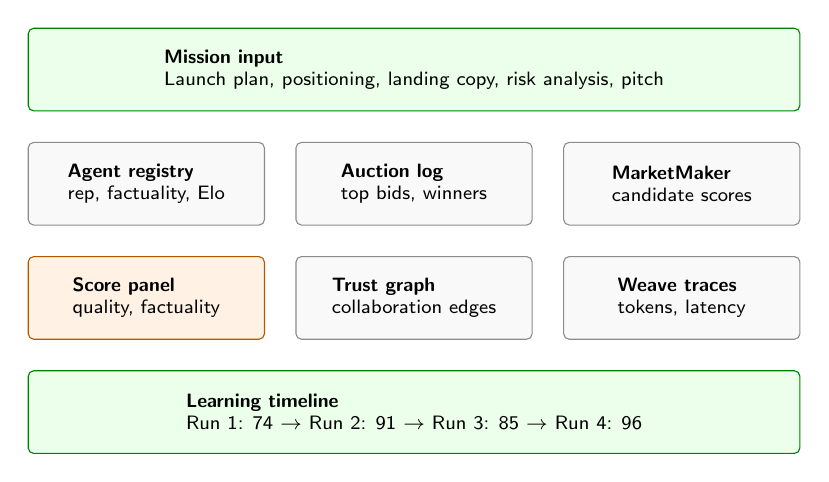
\begin{tikzpicture}[
  font=\sffamily\scriptsize,
  panel/.style={draw=black!45, fill=gray!5, rounded corners=2pt, minimum height=1.05cm, align=left},
  accent/.style={draw=green!50!black, fill=green!8, rounded corners=2pt, minimum height=1.05cm, align=left},
  warn/.style={draw=orange!70!black, fill=orange!10, rounded corners=2pt, minimum height=1.05cm, align=left}
]
\node[accent, minimum width=9.8cm, anchor=west] (mission) at (0,0) {\textbf{Mission input}\\Launch plan, positioning, landing copy, risk analysis, pitch};
\node[panel, minimum width=3.0cm, anchor=west] (registry) at (0,-1.45) {\textbf{Agent registry}\\rep, factuality, Elo};
\node[panel, minimum width=3.0cm, anchor=west] (auction) at (3.4,-1.45) {\textbf{Auction log}\\top bids, winners};
\node[panel, minimum width=3.0cm, anchor=west] (decision) at (6.8,-1.45) {\textbf{MarketMaker}\\candidate scores};
\node[warn, minimum width=3.0cm, anchor=west] (score) at (0,-2.9) {\textbf{Score panel}\\quality, factuality};
\node[panel, minimum width=3.0cm, anchor=west] (trust) at (3.4,-2.9) {\textbf{Trust graph}\\collaboration edges};
\node[panel, minimum width=3.0cm, anchor=west] (trace) at (6.8,-2.9) {\textbf{Weave traces}\\tokens, latency};
\node[accent, minimum width=9.8cm, anchor=west] (timeline) at (0,-4.35) {\textbf{Learning timeline}\\Run 1: 74 \(\rightarrow\) Run 2: 91 \(\rightarrow\) Run 3: 85 \(\rightarrow\) Run 4: 96};
\end{tikzpicture}
